\documentclass[conference]{IEEEtran}

\usepackage{graphicx}
\usepackage{multirow}
\usepackage{amsmath, amssymb}
\usepackage{hyperref}
\usepackage{caption}
\usepackage{cite}
\usepackage{float}
\usepackage{algorithm}
\usepackage{algorithmic}

\title{D.I.A.G.R.A.M.: Development of Image Analysis for Graph Recognition And Modeling}

\author{
    \IEEEauthorblockN{Filippo Garagnani, Saverio Napolitano, Nicola Ricciardi}
    \IEEEauthorblockA{
        'Computer Vision and Cognitive System' course \\
        \textit{Università di Modena e Reggio Emilia}
    }
}

\begin{document}

\maketitle

\begin{abstract}
This report describes D.I.A.G.R.A.M., a system for diagram recognition and generation. We present its architecture, the logic behind deterministic algorithms and the training of its deep learning components. The project aims to transform visual diagram input into structured representations.
\end{abstract}

\section{Introduction}
Diagrams are crucial in education, documentation, and many other fields. Developing a system that automatically understands and generates diagrams may reveal helpful for having high-quality, easily editable representations. This, however, poses challenges involving classification, shape detection, structure interpretation and symbolic representation. Our project proposes a modular architecture to tackle these tasks.

\section{Previous Works}
\cite{arrowrcnn} \\
\cite{interactiveUML} \\
\cite{sketchdiagram}

% System Architecture
\section{System Architecture}
Figure~\ref{fig:pipeline} illustrates the full pipeline, composed of four main modules: the Classifier, Extractor, Transducer, and Compiler. Each module is designed to process and transform the handwritten diagram image progressively toward a structured output.

\begin{figure}[H]
\centering
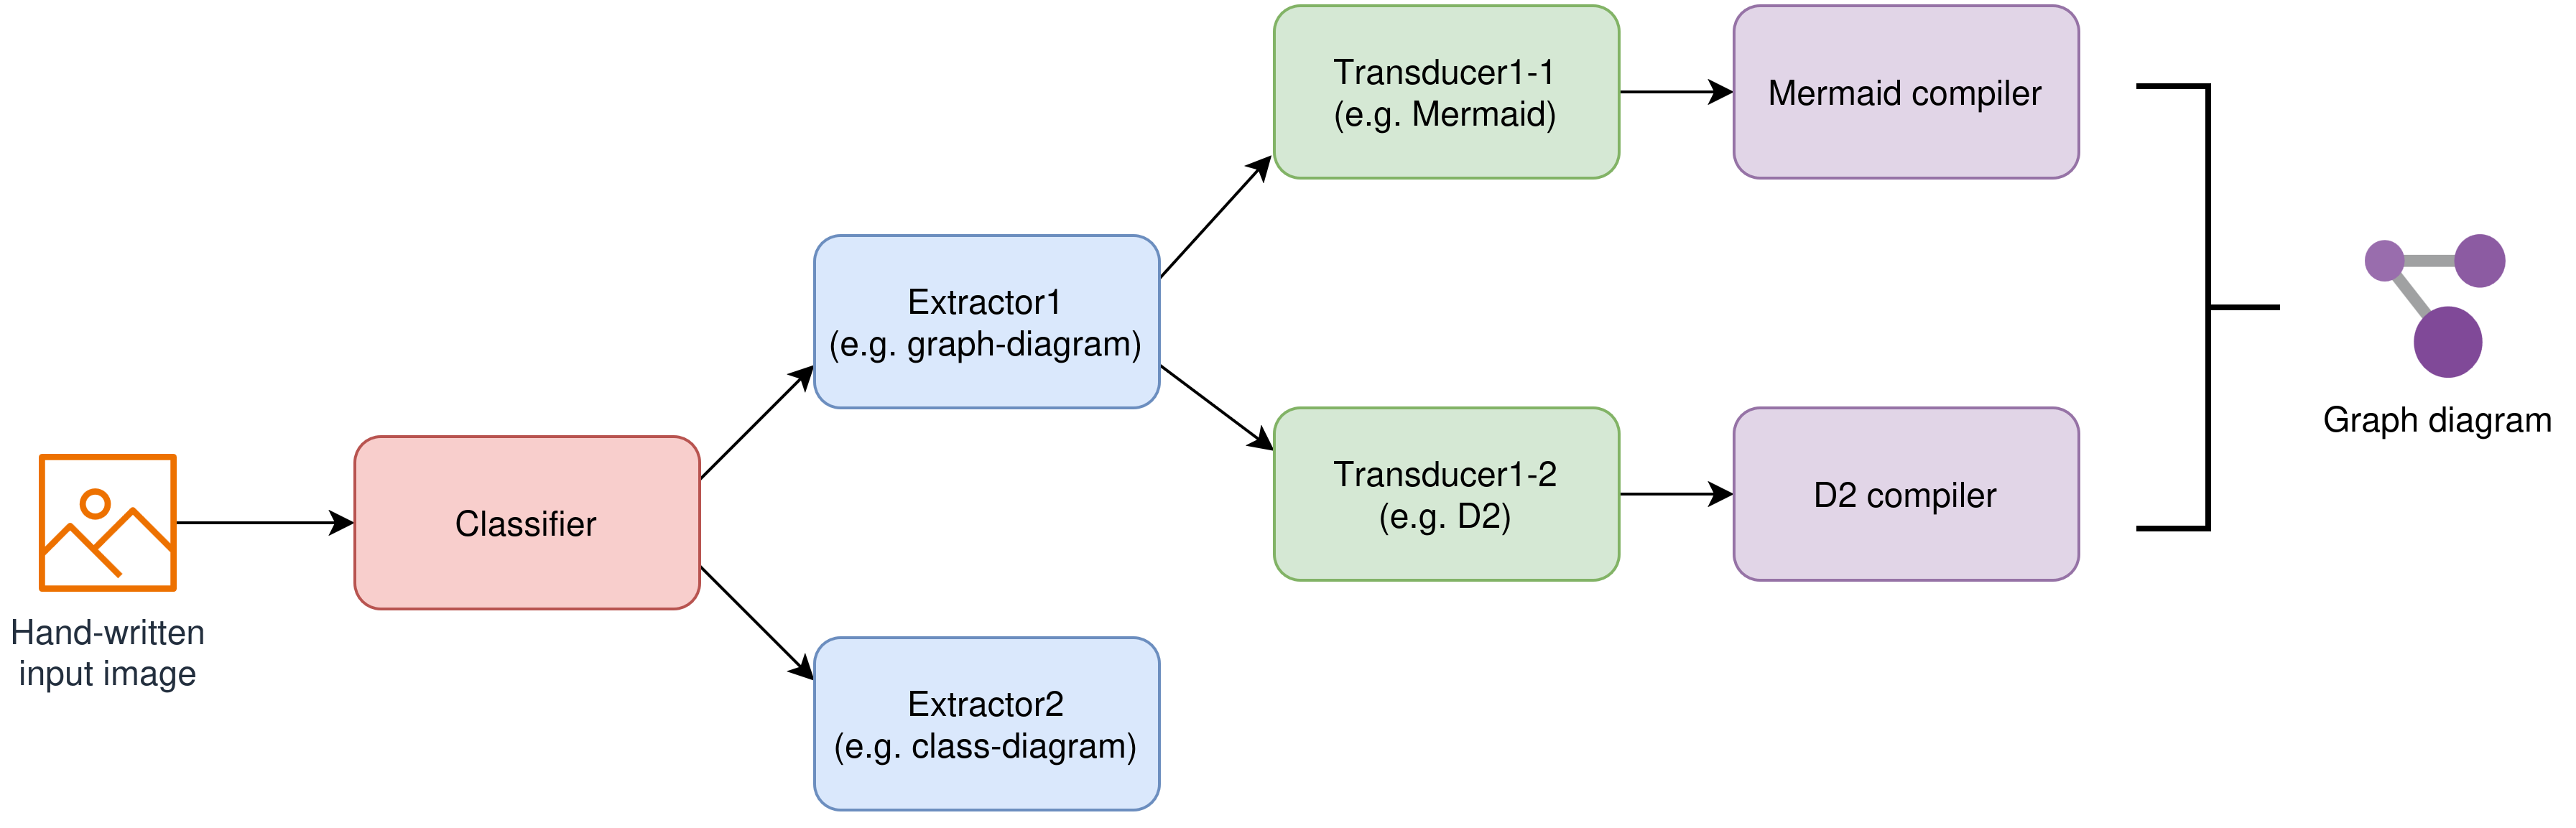
\includegraphics[width=\linewidth]{overview.png}
\caption{Overview of the D.I.A.G.R.A.M. system architecture.}
\label{fig:pipeline}
\end{figure}

The Classifier is able to recognize the category of the hand-written diagram that the user submitted as input. This is necessary in order for the system to know to which Extractor pass the data. This module is able to apply object detection and semantic recognition to represent the diagram in a unified way. After that, the representation is sent to the Transducer, which converts the data in a Markup language of choice. The Markup language content is therefore sent to the Compiler, thus generating the high-quality and editable diagram in .png format.

\subsection{Classifier Module}
The Classifier is the first component of the pipeline. It is able to tell to which category a given image of an handwritten diagram belongs to. This is necessary in order to later know the Extractors that can process the input image.
\subsection{Extractor Module}
The Extractor is the key component of the D.I.A.G.R.A.M. system, able to transform the raw diagram image into a structured, category-agnostic representation.
The Extractor recognizes the diagram's components, such as shapes, lines, and text, through an object detection network, and organizes them into a unified format. This representation serves as the foundation for the subsequent Transducer module, which converts the structured data into a domain-specific markup language.
\subsection{Transducer Module}
The Transducer is responsible for converting the unified, agnostic representation of a diagram into a domain-specific markup language. 
This transformation enables the subsequent Compiler module to generate high-quality visual outputs.
\subsection{Compiler Module}
The Compiler module is the final stage of the D.I.A.G.R.A.M. pipeline. 
Its primary role is to take the structured representation of the diagram, expressed in a markup language (e.g., Mermaid.js), and generate a high-quality diagram in a visual format such as PNG. 

% 
% Flowchart Diagram
%
\section{Flowchart Diagram Recognition}

\subsection{Internal Representation}
In order to pass data through the components of the pipeline in a unified way, it was necessary to decide upon an internal representation of the flowchart diagram. It consists of \textbf{elements} and \textbf{relations}. The latter are linked to at least one element. Every element has a \textit{category} and possibly some \textit{inner} and \textit{outer text}. Every relation has a \textit{category} too, either a \textit{source} or \textit{target element} or both, and possibly \textit{text} related to it.

This internal representation is generated from the image provided by the user by the Extractor module, while it is parsed and converted to a markup language of choice by the Transducer. 

\subsection{Classifier Module}
\subsubsection{Preprocessing}
Due to the fact that various kinds of diagrams' images could be submitted to the system, it was decided to streamline a unified preprocessing pipeline in order to reduce the differences that our classifier model had to handle. A few problems were analyzed and the final preprocessing pipeline for the classifier module is composed of the following operators, in order:
\begin{itemize}
	\item \textbf{Gray Scaling}: In order to remove colors from images, which was deemed an useless information for classifying diagrams.
	\item \textbf{Otsu Thresholding}: To binarize the image and reducing the information to handle.
	\item \textbf{Median Filtering}: Some images in our dataset - and in the use-case - were taken on checkered notebooks. The application of a median filter, with kernel size equal to three, totally removed these.
	\item \textbf{Perspective Correction}: The diagrams' images, sometimes, didn't occupy the full photo frame. Finding four keypoints (if possible) and stretching the image helped to fully employ the frame.
	\item \textbf{Padding}: This was necessary in order to keep the same net for every image. Changes in resolution would have implied changes in the number of paramters of the MLP layers.
\end{itemize}

Figure~\ref{fig:classifier_preprocessing} shows the step-by-step process of preparing an input image for the network.

\begin{figure}[H]
	\centering
	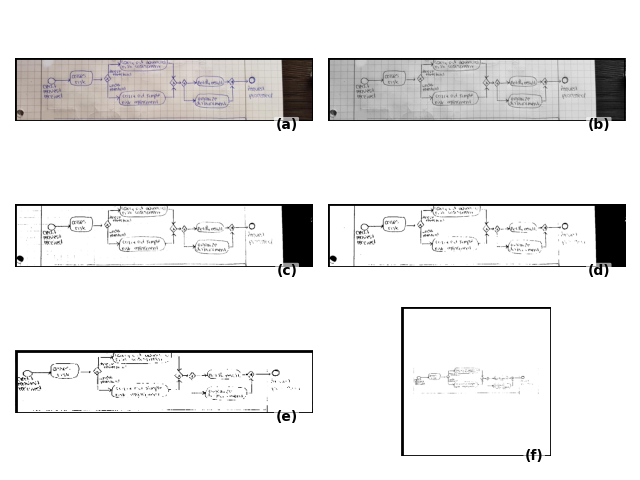
\includegraphics[width=250pt]{classifier_preprocessing.png}
	\caption{
		The operations applied by the preprocessing module.
		\textbf{(a)}: The raw image, still colored.
		\textbf{(b)}: The image in gray scale.
		\textbf{(c)}: The binarized image, thanks to Otsu.
		\textbf{(d)}: The median filter result. Some previous thin lines are now no more.
		\textbf{(e)}: The image with a perspective correction.
		\textbf{(f)}: The image in a standard size, ready to enter the network.
	}
	\label{fig:classifier_preprocessing}
\end{figure} 

\subsubsection{Model}
Since it was assumed that classifying two types of diagrams - with a third 'other' class - was a quite simple task, a small network was deemed enough. The model consists of three convolutional blocks - each containing a convolutional layer, followed by a batch normalization and a max-pooling layer - then followed by three linear layers (for a more detailed overview, see Appendix~\ref{classification_net}). The output vector of the MLP contains three features - one for each class that this specific classifier needs to address. In order to determine the prediction, the softmax function is then applied. As later seen in section~\ref{exp:classifier}, a weighted Cross-Entropy loss is then used to train the model.  \\

\subsection{Extractor Module}

\begin{figure}[H]
	\centering
	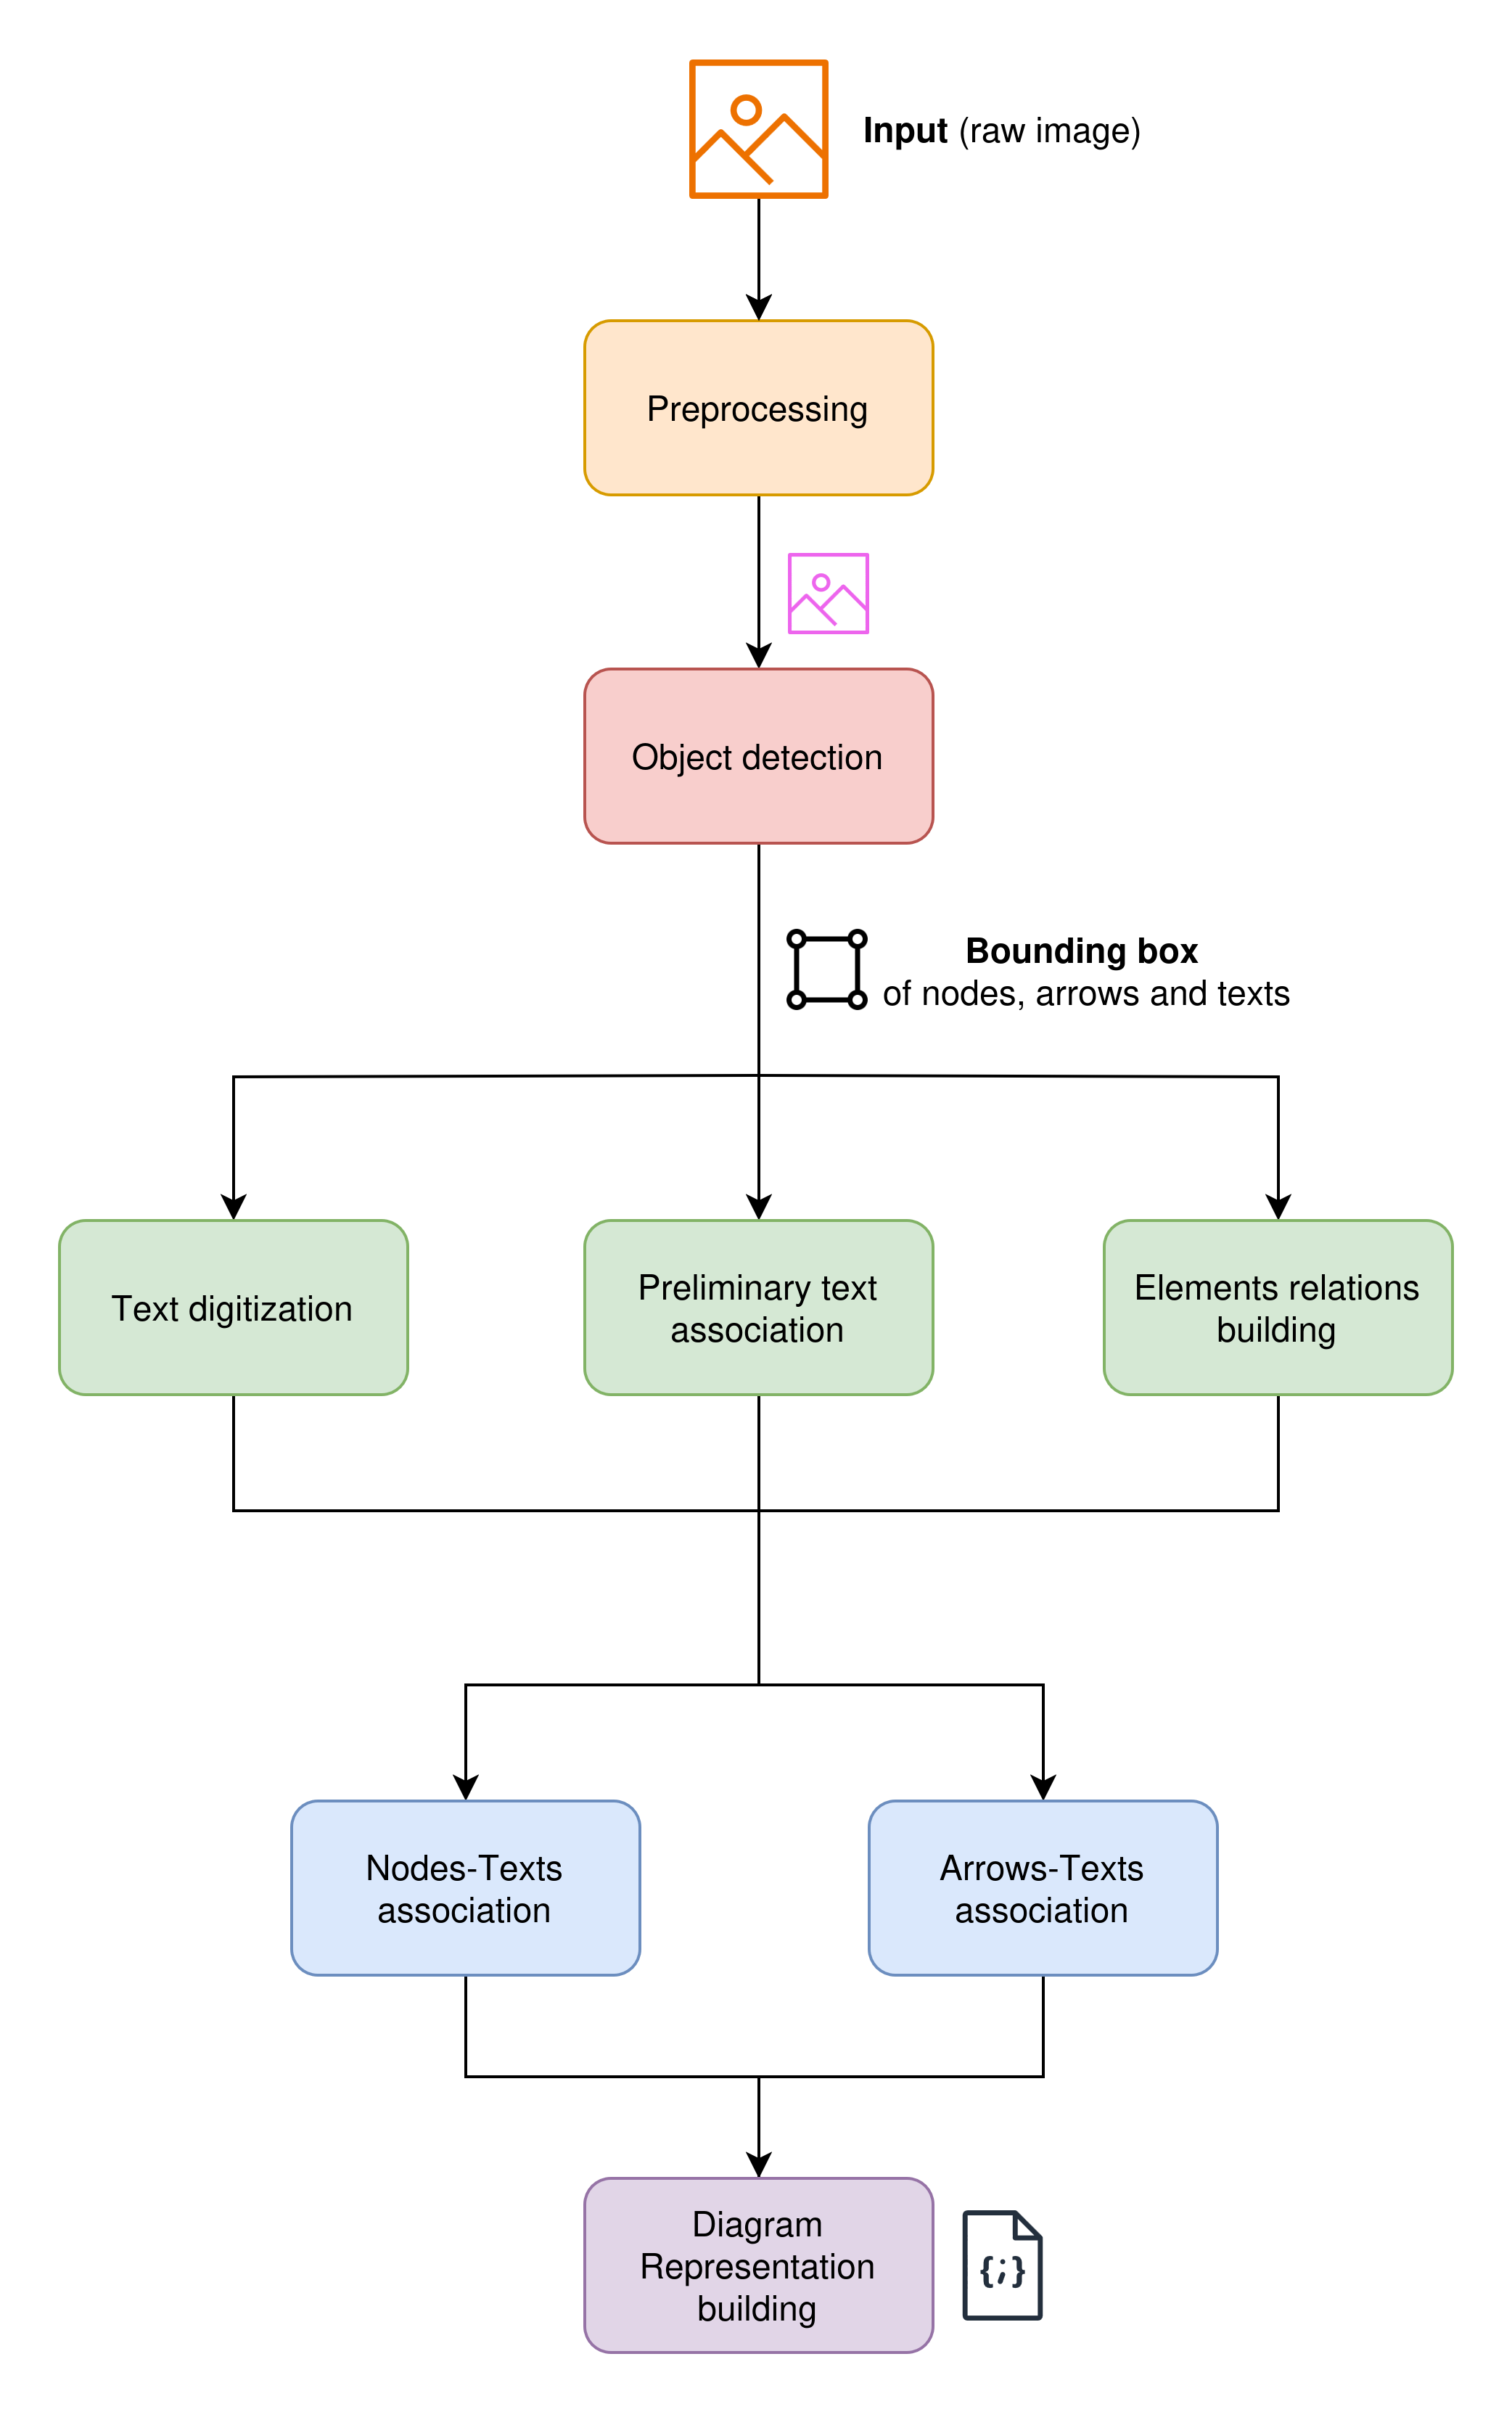
\includegraphics[width=\linewidth]{flowchart-extractor.png}
	\caption{The complete pipeline of the extractor module.}
	\label{fig:flowchart-extractor}
\end{figure}

\subsubsection{Preprocessing}
After some brief experiments, we found out that the object detection task through bounding boxes worked very well without any preprocessing technique. Moreover, the use of certain filters actually \textit{downgraded} the performances - e.g. the use of aggressive median filters reduced the capacity of the OCR model for text extraction.

The only preprocessing applied is a gray-scale transformation. Other transformations are not deemed necessary - the model employed automatically resize the input image, so it's not needed to do it beforehand. \\

\subsubsection{Bounding Box Detection}
\label{extr:bbd}
TODO: FasterRCNN - backbone ResNet 50FPN~\cite{rcnn}.  \\ After having determined all the bounding boxes of the diagram image, in order to correctly create the diagram internal representation, there's the need to link together text, elements and relations.\\


\subsubsection{Arrow Orientation}
To later correctly assign arrows to their source and target elements, the need to determine where the tip of an arrow lies. This task involves a few problems, among which determining exactly the arrow shape and its end - because sometimes other pen signs may be found in the bounding box of the arrow itself. After a few trials (and errors; for further insight, refer to section~\ref{exp:arrow_orientation}), the approach yielding the best results was through the use of the object detection network (see section~\ref{extr:bbd}) to recognize both arrow heads and tails. \\

\subsubsection{Text Digitization}
Since the task of converting an image of text into the relative string has already been solved in various ways, we settled upon the Microsoft \textit{Trocr Handwritten} Transformer model; more precisely, the \textit{base} version of it \cite{microsofttrocr}. Every bounding box containing text that has been found is later passed to the model, and the resulting string generated by the model is linked to it.\\

\subsubsection{Relationships Building}
Once the text has been digitized, it's necessary to effectively compute which elements are connected by which arrows. This is done by finding, for each arrow, the elements nearer to the head (which we will assume to be the 'target' of the relation) and to the tail (the 'source' of the relationship exemplified by the arrow). These associations are nullified if the distance is above a certain adjustable threshold. This last step is done under the hypothesis that an arrow may come from nothing - or may point to nothing, having actually only either the source or the target. \\

\subsubsection{Text Association}
It can be assumed that every piece of text is linked to one and only one element or relation. So, every bounding box containing text is linked to the nearest element - it being either a relation or an element. The associations that require too long a distance are eliminated further in the algorithm, and the relevant text is discarded.\\

\subsubsection{Element-Text Association}
After that a text box has been assigned to an element, there's the need to understand if the text is either inside or outside the element and whether the text is actually referring to the given element or not. In order to do this, the overlap between the two bounding boxes is computed; if the overlap is over a certain threshold, heuristically decided, the association is kept. Otherwise, the distance between the two bounding boxes is computed - as the distance between their central point. If the distance is over a certain threshold, the association is kept; otherwise, it's discarded.\\

\subsubsection{Relation-Text Association}
After a text box is assigned to a relation, some computation is needed to fully understand how the text is associated to the relation itself. The relation's bounding box is then split into three different sections. The overlap between the text bounding box and each of the three sections boxes is computed - then, the section with the highest overlap value is then assigned to the text under consideration. 

\section{Dataset}
TODO: Elencare i dataset usati, in che modo erano usati originariamente e come lo usiamo noi (quali dati per quali componenti) \\

\section{Experiments}

\subsection{Classifier}
\label{exp:classifier}
The first architecture explored for the Classifier module was a Convolutional Neural Network (CNN) following AlexNet's architecture, but smaller in size.
It had two Convolutional layers, each followed by a batch normalization and then by a max pooling layers. The first layer had only 4 filters, while the second one had 8.
The output of the second layer was then flattened and passed through a fully connected layer which downsized the features to 128, followed by a ReLU activation function. Other two fully connected layer brought the number of output features down to the number of classes.
Then, a softmax activation function was applied to the output layer, in order to obtain the probabilities of each class.
The model was trained on our own dataset, with only three possible output classes: 'flowchart', 'graph' and 'other'; it was trained for 10 epochs, with an AdamW optimizer (with a learning rate of 1e-3) and a standard CrossEntropy Loss function.
\\

We first tried such a small network because the features that had to be recognized were very simple, down to the basic shapes of the diagram elements.
However, the results showed a non-decreasing value of the loss function of 0.9 - better than $-ln(3) \simeq 1.1$, which is random guessing, but still not satisfactory.
\\

Judging this to be a problem in architecture size, we then tried adding another CNN layer with 16 filters; this one too followed by a batch normalization and a max pooling layer.
The rest of the net was untouched; we also decreased the learning rate to 1e-4, in order to avoid overshooting the minimum of the loss function.
The results, however, didn't show any kind of improvement, with the loss function still being around 0.9.
\\

While analyzing the predictions, we came up with what was actually the problem: the dataset was heavily unbalanced, with the 'other' class being the most represented one, shadowing the other two classes.
In order to solve this problem, we decided to use a weighted CrossEntropy Loss function, with the weights being inversely proportional to the number of samples in each class.

\begin{algorithm}
	\caption{Cross-Entropy weight computation}
	\begin{algorithmic}[1]
		\REQUIRE The classes' frequencies $f_1$, $f_2$, ..., $f_c$
		\STATE $S \gets \sum_{i = 1}^c f_i$
		\STATE $f_i \gets (f_i / S)^{-1}$
		\STATE $S \gets \sum_{i = 1}^c f_i$
		\STATE $f_i \gets f_i / S$
		\RETURN $f_1$, $f_2$, ..., $f_c$
	\end{algorithmic}
\end{algorithm}

This final approach showed a significant improvement in the results, with the loss function decreasing to around 0.6 after 10 epochs of training, with a global accuracy score of 97\% in the validation set.

\subsection{Object Detection}
TODO

\subsection{Arrow Orientation}
\label{exp:arrow_orientation}
As we've seen in the previous section, the need to find the exact position of an arrow's head arises (see \textbf{Appendix~\ref{double_clustering} and \textbf{Appendix}~\ref{arrow-net}} for a full overview of the first approaches).

The solution, as stated before, was to finetune the already working RCNN in order for it to also extract the bounding boxes of both tails and heads of the arrow.

\subsection{Text Digitization}
In order to choose an appropriate model, some tests were done over our specific dataset employing some different, pre-made models. The average results over the dataset are shown in Table~\ref{tab:text_digitization}.

\begin{table}[htbp]
\caption{Text Distance Metrics}
\centering
\begin{tabular}{lccc}
\hline
\textbf{Model} & \textbf{Hamming} & \textbf{Cosine} & \textbf{Euclidean} \\
\hline
microsoft-trocr-small-printed & 1.392 & 0.150 & 7133 \\
% microsoft-trocr-base-printed & 1.286 & 0.081 & 3594 \\
microsoft-trocr-small-handwritten & \textbf{1.346} & 0.100  & 3947 \\ 
\hline 
\textbf{microsoft-trocr-base-handwritten} & 1.549 & \textbf{0.057} & \textbf{3003} \\
\hline
\end{tabular}
\label{tab:text_digitization}
\end{table}

Some examples of the different models applied to our flowchart diagram dataset can be seen in Figure~\ref{fig:text_digitization_results_1} and in Figure~\ref{fig:text_digitization_results_2}.

\begin{figure}[H]
\centering
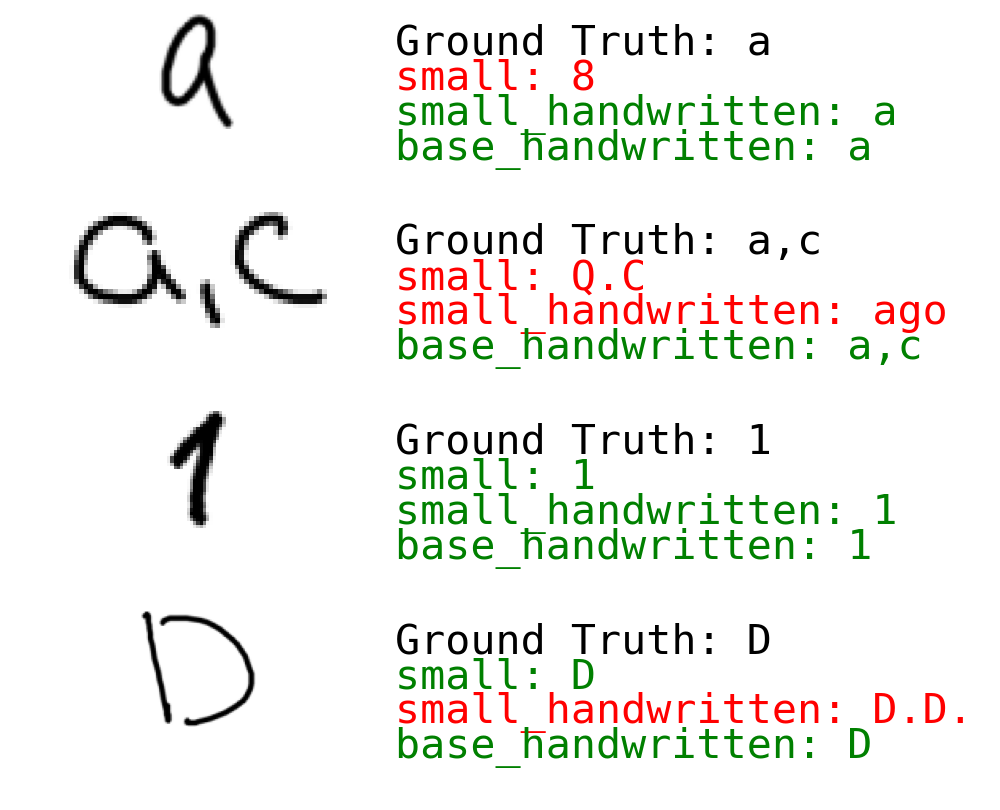
\includegraphics[width=\linewidth]{text_digitization_results_1.png}
\caption{Some random results of the text digitization over the proposed models.}
\label{fig:text_digitization_results_1}
\end{figure}

\begin{figure}[H]
\centering
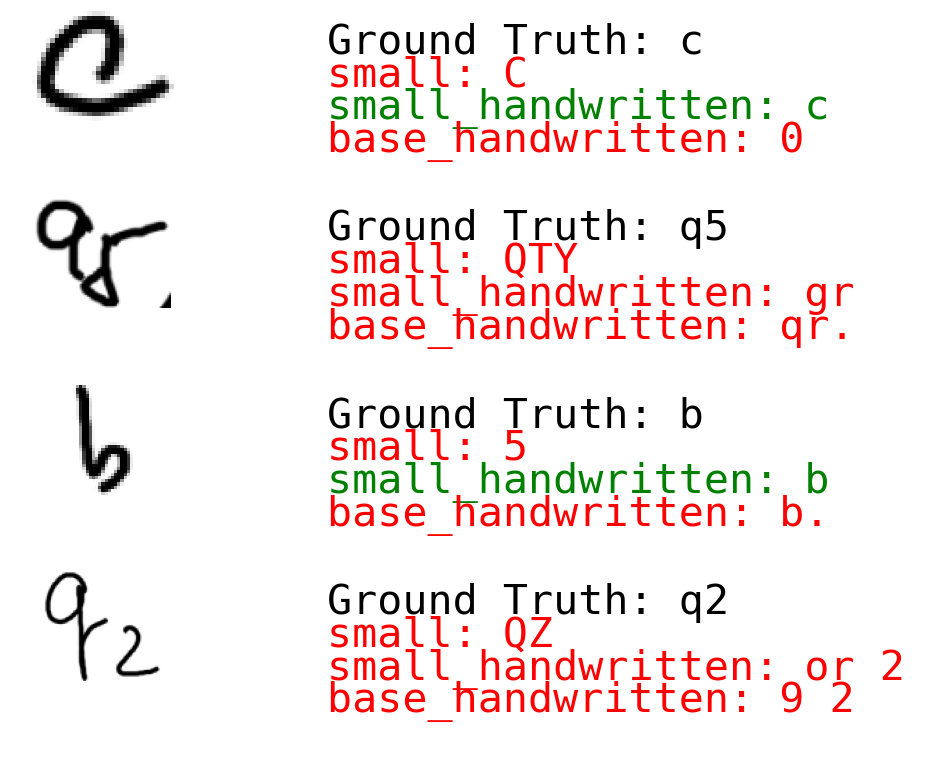
\includegraphics[width=\linewidth]{text_digitization_results_2.png}
\caption{Some results in which the \textit{trocr-base-handwritten} fails.}
\label{fig:text_digitization_results_2}
\end{figure}

\section{Discussion}
TODO

\section{Conclusion and Future Work}
TODO

\bibliographystyle{IEEEtran}

\newpage
\bibliography{article}
\newpage

\begin{appendices}

\section{Double Clustering}
\label{double_clustering}
The first algorithmic approach proposed to solve this task - called \textit{Double Clustering} - was as follows: 
\begin{enumerate}
	\item Apply a clustering algorithm to the bounding box.
	\item Suppose that the biggest cluster belongs to the arrow; the other clusters are thought to contain useless elements for this task, and can be discarded.
	\item Find the keypoints of the arrow using SIFT \cite{SIFT}.
	\item Find the two keypoints inside the arrow with maximum distance. Assume that these two points are closely related to the two ends of the arrow.
	\item Run a template matching procedure inside the two clusters to find the head of the arrow.
\end{enumerate}

For Step (1), we tried to employ both Spectral Clustering (see Figure~\ref{fig:spectral_clustering}) and DBScan \cite{dbscan} (see Figure~\ref{fig:arrow_double_clustering_clusters}).

\begin{figure}[H]
	\centering
	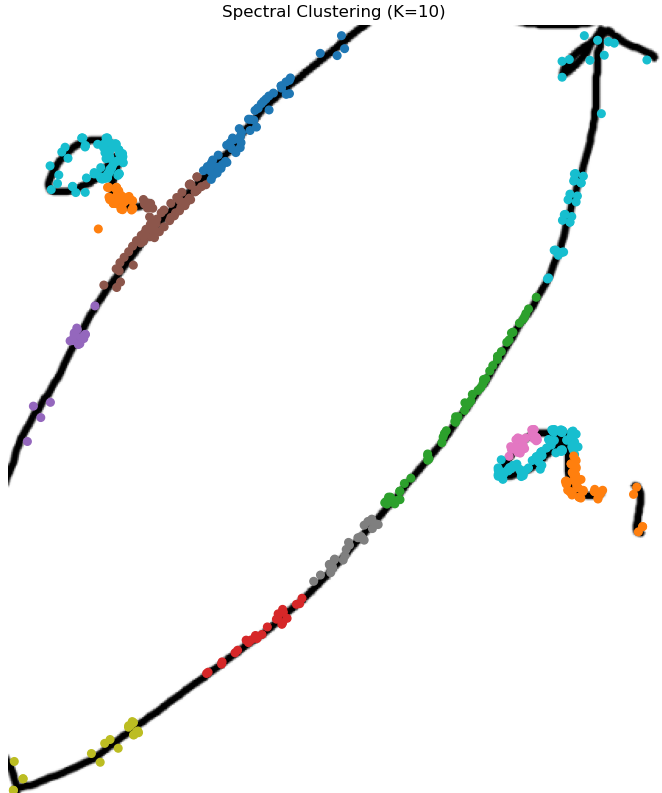
\includegraphics[width=150pt]{spectral_clustering.png}
	\caption{The result of Spectral Clustering to one instance of an arrow bounding box in our dataset.}
	\label{fig:spectral_clustering}
\end{figure}

\begin{figure}[H]
	\centering
	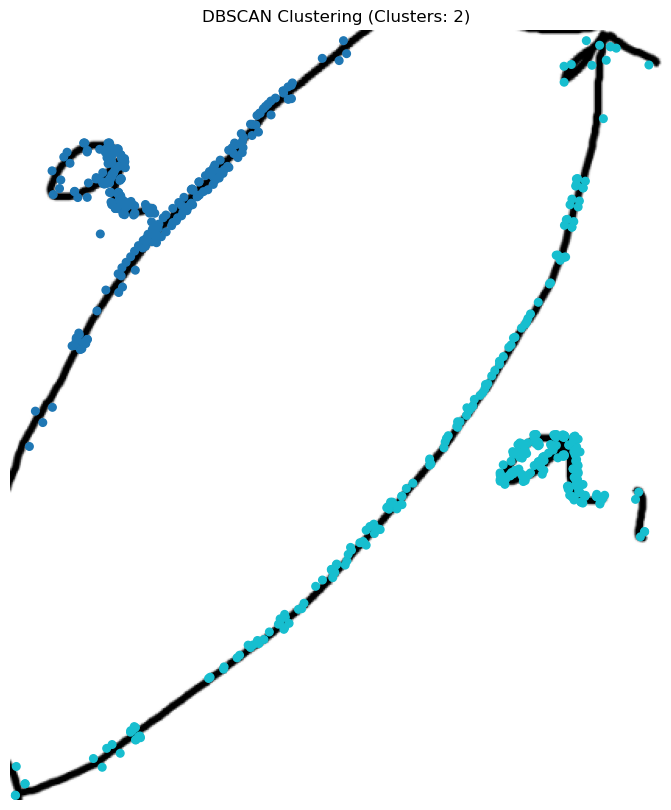
\includegraphics[width=150pt]{arrow_double_clustering_clusters.png}
	\caption{The result of DBScan to one instance of an arrow bounding box in our dataset.}
	\label{fig:arrow_double_clustering_clusters}
\end{figure}

For Step (3), we used SIFT \cite{SIFT} in order to find keypoints and some descriptors for them - necessary for the later template matching.
During Step (4), we were able to correctly deduce the overall direction of the arrow (see Figure~\ref{fig:arrow_double_clustering_direction}).

\begin{figure}[H]
	\centering
	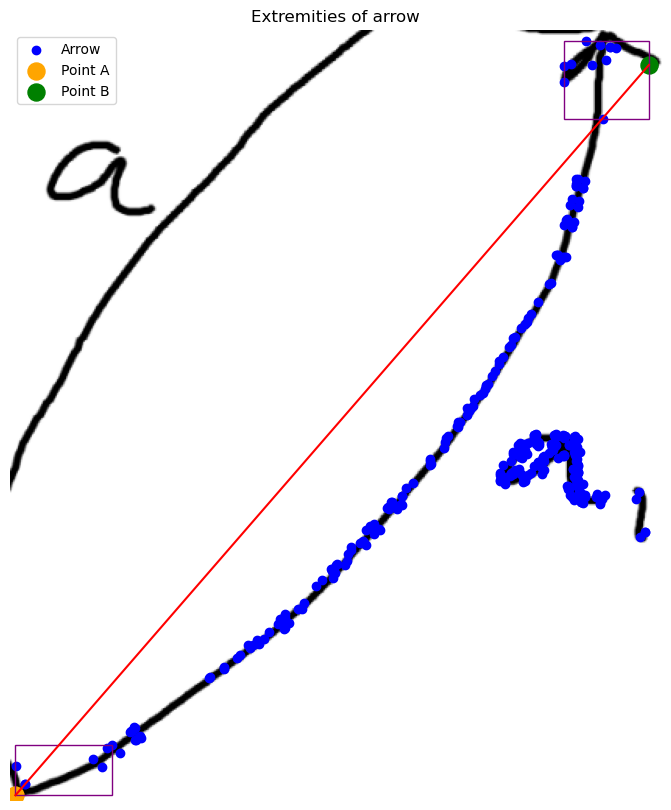
\includegraphics[width=150pt]{arrow_double_clustering_direction.png}
	\caption{The estimated direction of the arrow, finding the points that maximize the distance inside the cluster.}
	\label{fig:arrow_double_clustering_direction}
\end{figure}

For Step (5), we had previously hand-picked some templates (see Figure~\ref{fig:templates}).

\begin{figure}[H]
	\centering
	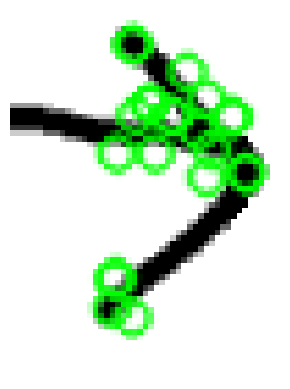
\includegraphics[width=50pt, height=60pt]{templates.png}
	\caption{An example of hand-picked template with SIFT descriptors.}
	\label{fig:templates}
\end{figure}

However, this approach didn't work as expected (see Figure~\ref{fig:template_matching_fail}). In particular, it never worked around self arrows: the maximized distance inside one of the two clusters is never between the tail and the head of the arrow.

\begin{figure}[H]
	\centering
	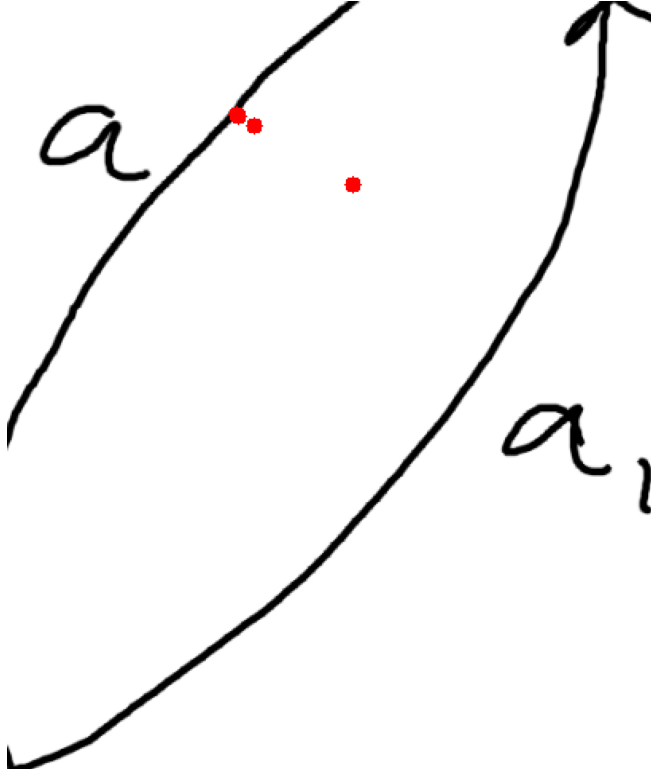
\includegraphics[width=150pt]{template_matching_fail.png}
	\caption{The overall result of the algorithm.}
	\label{fig:template_matching_fail}
\end{figure}

\section{ArrowNet}
\label{arrow-net}

This second approach for determining an arrow's orientation was inspired by UNet \cite{unet}. The core idea was to segment an arrow's bounding box, and to use a specific CNN to try and determine the arrow's head point and the arrow's tail point. The downsampling-upsampling network is called \textbf{ArrowNet} and its specifics can be found in Table~\ref{table:arrownet}.

\begin{table}[htbp]
	\centering
	\caption{ArrowNet Architecture Details}
	\label{tab:arrownet}
	\begin{tabular}{|l|l|l|l|l|}
		\hline
		\textbf{Stage} & \textbf{Layer} & \textbf{Out Channels} & \textbf{Operations} \\
		\hline
		\multirow{3}{*}{Encoder} 
		& Encoder1 & $32$ & Double Conv Block \\
		& MaxPool & $32$ & $2 \times 2$ MaxPooling \\
		& Encoder2 & $64$ & Double Conv Block \\
		\hline
		Bottleneck 
		& MaxPool + Bottleneck & $128$ & MaxPool + Double Conv \\
		\hline
		\multirow{4}{*}{Decoder}
		& Upsampling2 & $64$ & Transpose Conv Block \\
		& Skip + Decoder2 & $64$ & Concat + Double Conv \\
		& Upsampling1 & $32$ & Transpose Conv Block \\
		& Skip + Decoder1 & $32$ & Concat + Double Conv \\
		\hline
		Output & Output Conv & $3$ & $1 \times 1$ Convolution \\
		\hline
	\end{tabular}
	\label{table:arrownet}
\end{table}


\section{The Classification Network}
\label{classification_net}

\begin{table}[h]
	\centering
	\caption{Classification Network Details}
	\label{tab:classification-architecture}
	\begin{tabular}{|c|c|c|c|}
		\hline
		\textbf{Conv Layer} & \textbf{Output Channels} & \textbf{Kernel Size} & \textbf{Pool Kernel Size} \\
		\hline 
		1 & 8 & 2 & 3 \\
		2 & 16 & 2  & 3 \\
		3 & 24 & 3  & 2 \\
		\hline
		\textbf{Linear Layer} & \textbf{Output Features} & \textbf{Droput Rate} & \textbf{Activation Function} \\
		\hline 
		1 & 2048 & 0.2 & ReLU \\
		2 & 128 & 0.2 & ReLU \\
		3 & 3 & 0.2 & ReLU \\
		\hline
	\end{tabular}
\end{table}

\end{appendices}

\end{document}
